\chapter{\uppercase{Methodology}}

\section{Maximum Principles}
%================================================================================
\subsection{Integral Form of the Time-Dependent Transport Equation}
%================================================================================
\begin{theorem}{Exact Solution to Time-Dependent Transport Equation}
   An implicit solution to the initial value problem
   \begin{equation}\label{PDE}
      \frac{\partial \psi}{\partial t} + c\mathbf{\Omega}\cdot\nabla\psi(\mathbf{x},t)
      + c\sigma(\mathbf{x})\psi(\mathbf{x},t) = c q(\mathbf{x},t),
      \qquad \psi(\mathbf{x},0) = \psi_0(\mathbf{x})
   \end{equation}
   is the following:
   \begin{equation}\label{exact}
      \psi(\mathbf{x},t) = \psi_0(\mathbf{x} - c\mathbf{\Omega}t)
         e^{-c\int\limits_0^t \sigma(\mathbf{x} - c\mathbf{\Omega}(t -t'))dt'} +
         c \int\limits_0^t q(\mathbf{x} - c\mathbf{\Omega}(t -t'),t')
         e^{-c\int\limits_{t'}^t\sigma(\mathbf{x}
         - c\mathbf{\Omega}(t -\bar{t}))d\bar{t}} dt'.
   \end{equation}
\end{theorem}

\begin{proof}
   This proof will proceed by using the Method of Characteristics. The position
   $\mathbf{x}$ will be regarded as a function of time: $\mathbf{x}=\mathbf{x}(t)$.
   The characteristic $\mathbf{x}(t)$ is the solution of the following initial value problem:
   \[
      \frac{d\mathbf{x}}{dt} = c\mathbf{\Omega},\qquad \mathbf{x}(0) = \mathbf{x}_0,
   \]
   which is
   \[
      \mathbf{x}(t) = \mathbf{x}_0 + c\mathbf{\Omega}t.
   \]
   Taking the derivative of $\psi(\mathbf{x}(t),t)$ gives
   \begin{eqnarray*}
      \frac{d\psi}{dt} & = &\frac{\partial\psi}{\partial t} +
      \nabla\cdot\psi(\mathbf{x}(t),t) \frac{d\mathbf{x}}{dt}\\
      & = &\frac{\partial \psi}{\partial t} +
      c\mathbf{\Omega}\cdot\nabla\psi(\mathbf{x}(t),t),
   \end{eqnarray*}
   which when combined with the PDE in Equation \eqref{PDE}, gives
   \[
      \frac{d\psi}{dt} + c\sigma(\mathbf{x}(t))\psi(\mathbf{x}(t),t) = c q(\mathbf{x},t).
   \]
   This is a 1st-order linear ODE, which may be solved using an integrating factor
   \[
      \mu(t)=e^{c\int\limits_0^t\sigma(\mathbf{x}(t'))dt'}.
   \]
   Multiplying both sides by this integrating factor and using the product rule,
   \[
      \frac{d}{dt}\left[\psi(\mathbf{x}(t),t)\mu(t)\right] = c q(\mathbf{x}(t),t) \mu(t),
   \]
   and integrating from $0$ to $t$ gives
   \[
      \psi(\mathbf{x}(t),t)\mu(t)-\psi(\mathbf{x}(0),0)\mu(0) =
         \int\limits_0^t c q(\mathbf{x}(t'),t') \mu(t') dt'.
   \]
   Simplifying,
   \[
      \psi(\mathbf{x}(t),t) = \psi(\mathbf{x}(0),0)
         e^{-c\int\limits_0^t \sigma(\mathbf{x}(t'))dt'} +
         \left(c \int\limits_0^t q(\mathbf{x}(t'),t')
         e^{c\int\limits_0^{t'}\sigma(\mathbf{x}(\bar{t}))d\bar{t}} dt'\right)
         e^{-c\int\limits_0^t\sigma(\mathbf{x}(t'))dt'},
   \]
   \[
      \psi(\mathbf{x}(t),t) = \psi(\mathbf{x}(0),0)
         e^{-c\int\limits_0^t \sigma(\mathbf{x}(t'))dt'} +
         c \int\limits_0^t q(\mathbf{x}(t'),t')
         e^{-c\int\limits_{t'}^t\sigma(\mathbf{x}(\bar{t}))d\bar{t}} dt'.
   \]
   Finally, expressing $\mathbf{x}(t)$ in terms of $\mathbf{x}$, $\mathbf{\Omega}$,
   and $t$ gives
   \[
      \psi(\mathbf{x},t) = \psi_0(\mathbf{x} - c\mathbf{\Omega}t)
         e^{-c\int\limits_0^t \sigma(\mathbf{x} - c\mathbf{\Omega}(t -t'))dt'} +
         c \int\limits_0^t q(\mathbf{x} - c\mathbf{\Omega}(t -t'),t')
         e^{-c\int\limits_{t'}^t\sigma(\mathbf{x}
         - c\mathbf{\Omega}(t -\bar{t}))d\bar{t}} dt'.\qed
   \]
\end{proof}
%--------------------------------------------------------------------------------
\subsection{Integral Form of the Steady-State Transport Equation}
%================================================================================
\begin{theorem}{Exact Solution to Steady-State Transport Equation}
   An implicit solution to the equation
   \begin{equation}\label{PDEss}
      \mathbf{\Omega}\cdot\nabla\psi(\mathbf{x})
      + \sigma(\mathbf{x})\psi(\mathbf{x}) = q(\mathbf{x})
   \end{equation}
   is the following:
   \begin{equation}\label{exactss}
      \psi(\mathbf{x}) = \psi(\mathbf{x} - s\mathbf{\Omega})
         e^{-\int\limits_0^s \sigma(\mathbf{x} - \mathbf{\Omega}(s -s'))ds'} +
         \int\limits_0^s q(\mathbf{x} - \mathbf{\Omega}(s -s'))
         e^{-\int\limits_{s'}^s\sigma(\mathbf{x}
         - \mathbf{\Omega}(s -\bar{s}))d\bar{s}} ds'.
   \end{equation}
\end{theorem}

\begin{proof}
   This proof will proceed by using the Method of Characteristics. The position
   $\mathbf{x}$ will be regarded as a function of position $s$ along the line
   with direction $\mathbf{\Omega}$ that passes through $\mathbf{x}$:
   \[
      \mathbf{x}(s) = \mathbf{x}_0 + \mathbf{\Omega}s.
   \]
   Using the chain rule,
   \[
      \frac{d\psi}{ds} = \nabla\psi(\mathbf{x}(s)) \cdot \frac{d\mathbf{x}}{ds}
         = \mathbf{\Omega} \cdot \nabla\psi(\mathbf{x}(s)),
   \]
   which when combined with the PDE in Equation \eqref{PDEss}, gives
   \[
      \frac{d\psi}{ds} + \sigma(\mathbf{x}(s))\psi(\mathbf{x}(s)) = q(\mathbf{x}(s)).
   \]
   This is a 1st-order linear ODE, which may be solved using an integrating factor
   \[
      \mu(s)=e^{\int\limits_0^s\sigma(\mathbf{x}(s'))ds'}.
   \]
   Multiplying both sides by this integrating factor and using the product rule,
   \[
      \frac{d}{ds}\left[\psi(\mathbf{x}(s))\mu(s)\right] = q(\mathbf{x}(s)) \mu(s),
   \]
   and integrating from $0$ to $s$ gives
   \[
      \psi(\mathbf{x}(s))\mu(s)-\psi(\mathbf{x}(0))\mu(0) =
         \int\limits_0^s q(\mathbf{x}(s')) \mu(s') ds'.
   \]
   Simplifying,
   \[
      \psi(\mathbf{x}(s)) = \psi(\mathbf{x}(0))
         e^{-\int\limits_0^s \sigma(\mathbf{x}(s'))ds'} +
         \left(\int\limits_0^s q(\mathbf{x}(s'))
         e^{\int\limits_0^{s'}\sigma(\mathbf{x}(\bar{s}))d\bar{s}} ds'\right)
         e^{-\int\limits_0^s\sigma(\mathbf{x}(s'))ds'},
   \]
   \[
      \psi(\mathbf{x}(s)) = \psi(\mathbf{x}(0))
         e^{-\int\limits_0^s \sigma(\mathbf{x}(s'))ds'} +
         \int\limits_0^s q(\mathbf{x}(s'))
         e^{-\int\limits_{s'}^s\sigma(\mathbf{x}(\bar{s}))d\bar{s}} ds'.
   \]
   Finally, expressing $\mathbf{x}(s)$ in terms of $\mathbf{x}$, $\mathbf{\Omega}$,
   and $s$ gives
   \[
      \psi(\mathbf{x}) = \psi(\mathbf{x} - \mathbf{\Omega}s)
         e^{-\int\limits_0^s \sigma(\mathbf{x} - \mathbf{\Omega}(s -s'))ds'} +
         \int\limits_0^s q(\mathbf{x} - \mathbf{\Omega}(s -s'))
         e^{-\int\limits_{s'}^s\sigma(\mathbf{x}
         - \mathbf{\Omega}(s -\bar{s}))d\bar{s}} ds'.\qed
   \]
\end{proof}
%--------------------------------------------------------------------------------
\subsection{Continuous Maximum Principles}
%================================================================================
\begin{theorem}[label={cont}]{Continuous Maximum Principle}
   The following continuous maximum principle is valid for the solution to the
   problem given by Equation \eqref{PDE}:
   \begin{equation}
      \psi_{\min,N}^0 e^{-c\tau\sigma_{\max,N}} + 
            \frac{q_{\min,N}}{\sigma_{\max,N}}(1 - e^{-c\sigma_{\max,N}\tau})
      \le\psi(\mathbf{x},\tau)\le
      \psi_{\max,N}^0 e^{-c\tau\sigma_{\min,N}} + 
            \frac{q_{\max,N}}{\sigma_{\min,N}}(1 - e^{-c\sigma_{\min,N}\tau}).
   \end{equation}
   where $\psi_{\max,N}^0\equiv\max\limits_{\mathbf{y}\in N(\mathbf{x})}\psi(\mathbf{y},0)$,
   $\sigma_{\max,N}\equiv\max\limits_{\mathbf{y}\in N(\mathbf{x})}\sigma(\mathbf{y})$, with
   $\psi_{\min,N}^0$ and $\sigma_{\min,N}$ defined similarly, and the neighborhood $N$ is a
   sphere centered at $\mathbf{x}$ with radius $c\tau$:
   \begin{equation}
      N(\mathbf{x})\equiv\left\{\mathbf{y}\in\mathbb{R}^d : 
         \|\mathbf{y} - \mathbf{x}\| \le c\tau\right\}.
   \end{equation}
\end{theorem}

\begin{proof}
   Rewriting Equation \eqref{exact} with $t=\tau$ gives
   \[
      \psi(\mathbf{x},\tau) = \psi_0(\mathbf{x} - c\mathbf{\Omega}\tau)
         e^{-c\int\limits_0^\tau \sigma(\mathbf{x} - c\mathbf{\Omega}(\tau -t'))dt'} +
         c \int\limits_0^\tau q(\mathbf{x} - c\mathbf{\Omega}(\tau -t'),t')
         e^{-c\int\limits_{t'}^\tau\sigma(\mathbf{x}
         - c\mathbf{\Omega}(\tau -\bar{t}))d\bar{t}} dt'.
   \]
   Let $L(\mathbf{x})$ be the line segment that spans between 
   $\mathbf{x}-c\mathbf{\Omega}\tau$ and $\mathbf{x}$:
   \[
      L(\mathbf{x})\equiv \left\{\mathbf{y}\in\mathbb{R}^d : \mathbf{y}
         = \mathbf{x}-ct\mathbf{\Omega},\qquad t\in(0,\tau) \right\}.
   \]
   One can bound the first term in the right hand side of Equation \eqref{exactss}
   as follows:
   \[
      \psi_{\min,L}^0 e^{-c\tau\sigma_{\max,L}} \le
      \psi_0(\mathbf{x} - c\mathbf{\Omega}\tau)
         e^{-c\int\limits_0^\tau \sigma(\mathbf{x} - c\mathbf{\Omega}(\tau -t'))dt'} \le
      \psi_{\max,L}^0 e^{-c\tau\sigma_{\min,L}},
   \]
   where $\psi_{\max,L}^0 \equiv\max\limits_{\mathbf{y}\in L(\mathbf{x})}\psi_0(\mathbf{y})$,
   $\sigma_{\max,L}\equiv\max\limits_{\mathbf{y}\in L(\mathbf{x})}\sigma(\mathbf{y})$,
   with $\psi_{\min,L}^0$ and $\sigma_{\min,L}$
   defined similarly.
   The source term can be bounded as follows:
   \begin{eqnarray*}
      c \int\limits_0^\tau q(\mathbf{x} - c\mathbf{\Omega}(\tau -t'),t')
         e^{-c\int\limits_{t'}^\tau\sigma(\mathbf{x}
         - c\mathbf{\Omega}(\tau -\bar{t}))d\bar{t}} dt' & \le &
         c q_{\max,L}\int\limits_0^\tau 
         e^{-c\int\limits_{t'}^\tau\sigma(\mathbf{x}
         - c\mathbf{\Omega}(\tau -\bar{t}))d\bar{t}} dt'\\
      & \le & c q_{\max,L}\int\limits_0^\tau 
         e^{-c\sigma_{\min,L}\int\limits_{t'}^\tau d\bar{t}} dt'\\
      & = & c q_{\max,L} \int\limits_0^\tau e^{-c\sigma_{\min,L}(\tau-t')} dt'\\
      & = & c q_{\max,L}e^{-c\sigma_{\min,L}\tau}
         \int\limits_0^\tau e^{c\sigma_{\min,L}t'} dt'\\
      & = & \left\{\begin{array}{l l}
            \frac{q_{\max,L}}{\sigma_{\min,L}}(1 - e^{-c\sigma_{\min,L}\tau})
               & \sigma_{\min,L} \ne 0\\
            c\tau q_{\max,L} & \sigma_{\min,L} = 0
            \end{array}\right.
   \end{eqnarray*}
   A similar analysis is performed for the lower bound. Putting everything together,
   the following is a maximum principle on $L(\mathbf{x})$:
   \[
      \psi_{\min,L}^0 e^{-c\tau\sigma_{\max,L}} + 
            \frac{q_{\min,L}}{\sigma_{\max,L}}(1 - e^{-c\sigma_{\max,L}\tau})
      \le\psi(\mathbf{x},\tau)\le
      \psi_{\max,L}^0 e^{-c\tau\sigma_{\min,L}} + 
            \frac{q_{\max,L}}{\sigma_{\min,L}}(1 - e^{-c\sigma_{\min,L}\tau}).
   \]
   Since $L(\mathbf{x})\subset N(\mathbf{x})$, the following is true:
   \[
      \psi_{\min,N}^0 e^{-c\tau\sigma_{\max,N}} + 
            \frac{q_{\min,N}}{\sigma_{\max,N}}(1 - e^{-c\sigma_{\max,N}\tau})
      \le\psi(\mathbf{x},\tau)\le
      \psi_{\max,N}^0 e^{-c\tau\sigma_{\min,N}} + 
            \frac{q_{\max,N}}{\sigma_{\min,N}}(1 - e^{-c\sigma_{\min,N}\tau}).\qed
   \]
\end{proof}
%--------------------------------------------------------------------------------
%\begin{theorem}{Upwind Continuous Maximum Principle}
   %The following continuous maximum principle is valid for the solution to the
   %problem given by Equation \eqref{PDE}:
   %\begin{equation}
      %\psi_{\min,N^-}^0 e^{-c\tau\sigma_{\max,N^-}} \le
      %\psi(\mathbf{x},\tau) \le
      %\psi_{\max,N^-}^0 e^{-c\tau\sigma_{\min,N^-}},
   %\end{equation}
   %where $\psi_{\max,N^-}^0\equiv\max\limits_{\mathbf{y}\in N^-(\mathbf{x})}
   %\psi(\mathbf{y},0)$, $\sigma_{\max,N^-}\equiv\max\limits_{\mathbf{y}\in N^-(\mathbf{x})}
   %\sigma(\mathbf{y})$, with $\psi_{\min,N^-}^0$ and $\sigma_{\min,N^-}$
   %defined similarly, and $N^-(\mathbf{x})$ is the upwind subset of $N(\mathbf{x})$:
   %\begin{equation}
      %N^-(\mathbf{x})\equiv\left\{\mathbf{y}\in N : (\mathbf{y} - \mathbf{x})\cdot \mathbf{\Omega} \le 0\right\}.
   %\end{equation}
%\end{theorem}
%\begin{proof}
   %The proof proceeds exactly as for Theorem \ref{cont}, except replacing $N$ with $N^-$.
%\end{proof}

Text goes here \cite{Agrawal1986}.

\section{New Section}

%%%%%%%%%%%%%%%%%%%%%%%%%%%%%%%%%%%%%%%%%%%%%%%%%%%%%%
\begin{figure}[H]
\centering
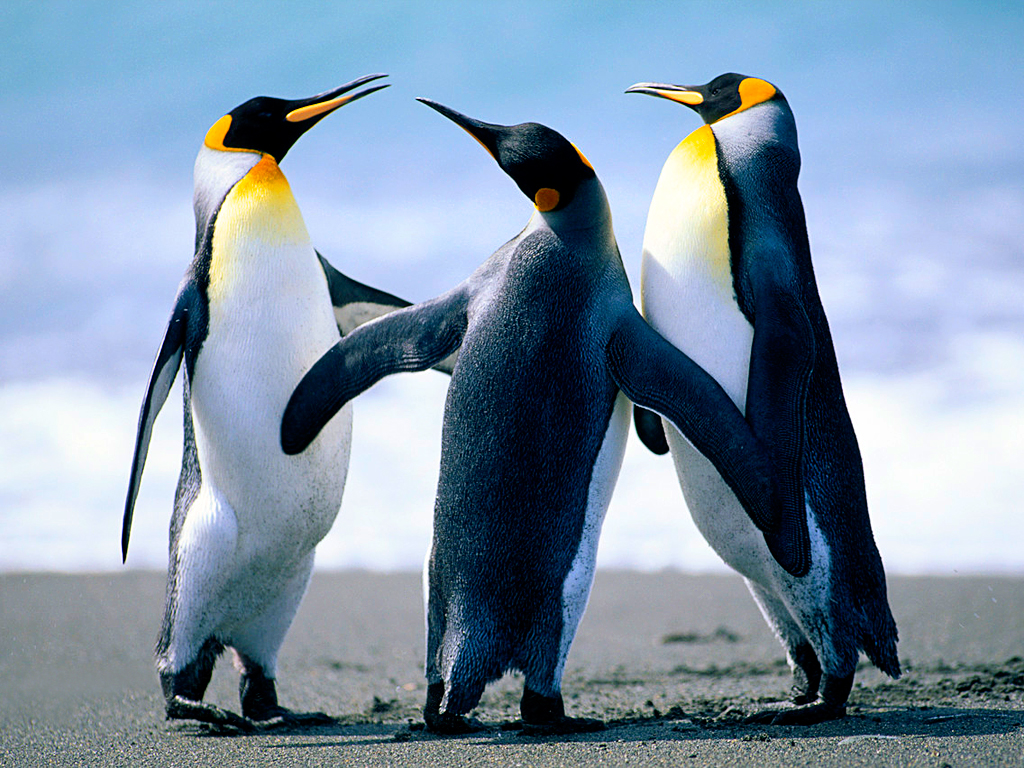
\includegraphics[scale=.50]{figures/Penguins.jpg}
\caption{TAMU figure}
\label{fig:tamu-fig3}
\end{figure}
%%%%%%%%%%%%%%%%%%%%%%%%%%%%%%%%%%%%%%%%%%%%%%%%%%%%%%
\section{Another Section}

Text between the figures.  Text between the figures. Text between the figures. Text between the figures.  Text between the figures. Text between the figures. Text between the figures.  Text between the figures. Text between the figures. Text between the figures.  Text between the figures. Text between the figures.
%%%%%%%%%%%%%%%%%%%%%%%%%%%%%%%%%%%%%%%%%%%%%%%%%%%%%%%
%\begin{figure}[H]
%\centering
%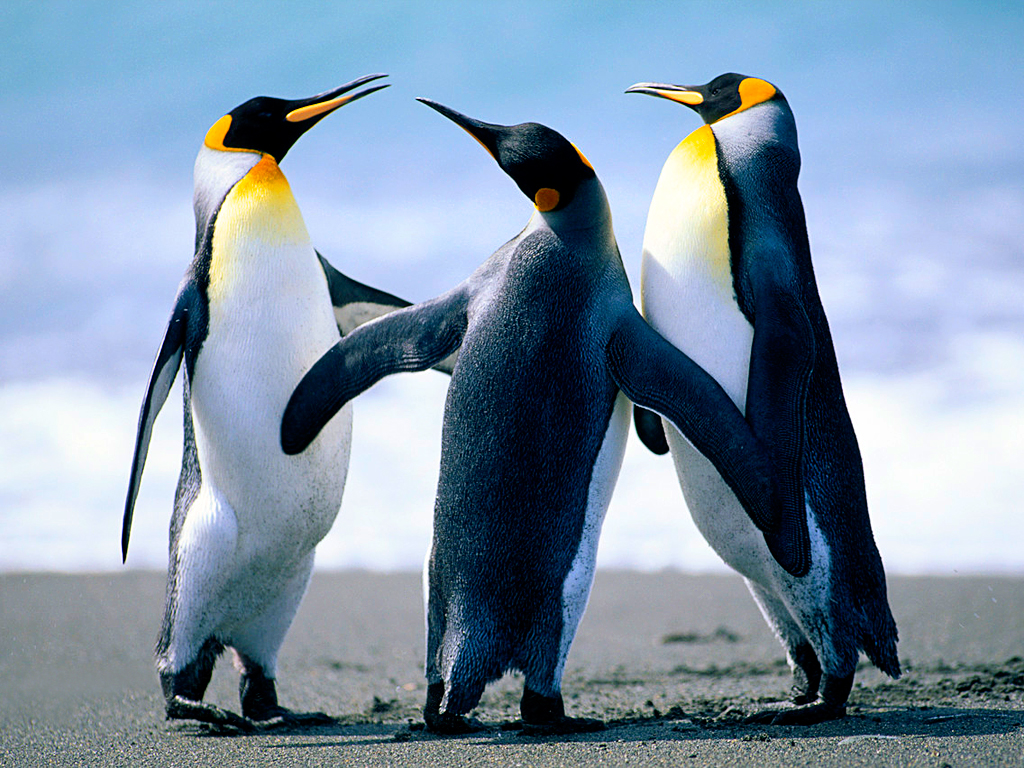
\includegraphics[scale=.50]{figures/Penguins.jpg}
%\caption{Another TAMU figure}
%\label{fig:tamu-fig4}
%\end{figure}
%%%%%%%%%%%%%%%%%%%%%%%%%%%%%%%%%%%%%%%%%%%%%%%%%%%%%%%

\subsection{Subsection}

%%%%%%%%%%%%%%%%%%%%%%%%%%%%%%%%%%%%%%%%%%%%%%%%%%%%%%%
%\begin{figure}[H]
%\centering
%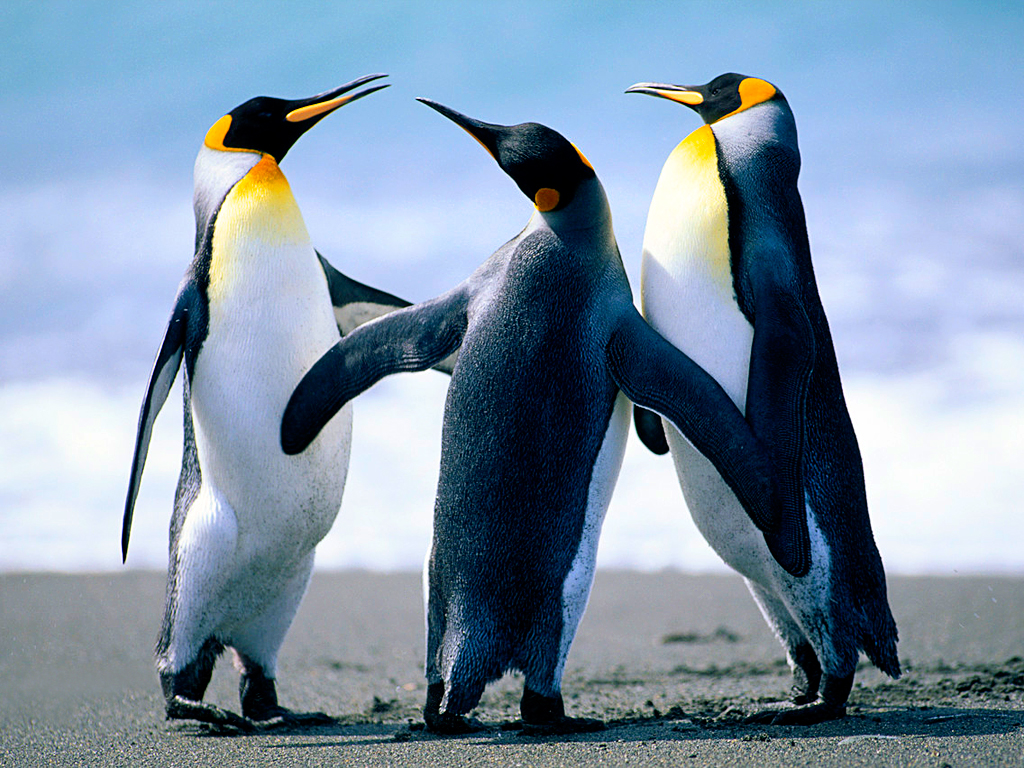
\includegraphics[scale=.50]{figures/Penguins.jpg}
%\caption{Another TAMU figure}
%\label{fig:tamu-fig4-2}
%\end{figure}
%%%%%%%%%%%%%%%%%%%%%%%%%%%%%%%%%%%%%%%%%%%%%%%%%%%%%%%
\subsection{Subsection}

A table example is going to follow.

\begin{table}[H]
\centering
\caption{This is a table template}
\begin{tabular}{|l|c|c|c|c|c|}
\hline
Product & 1 & 2 & 3 & 4 & 5\\
\hline
Price & 124.- & 136.- & 85.- & 156.- & 23.-\\
Guarantee [years] & 1 & 2 & - & 3 & 1\\
Rating & 89\% & 84\% & 51\% & & 45\%\\
\hline
\hline
Recommended & yes & yes & no & no & no\\
\hline
\end{tabular}
\label{tab:template2}
\end{table}
\section{Another Section}
